% 4.9
\begin{thSatz}
    Sei $X$ ein $\R$-Vektorraum, sei $f\colon X\to\R$ linear und sei
    $\alpha\in\R$.
    Die Hyperebene $H = \{ f=\alpha \}$ ist genau dann abgeschlossen, wenn $f$
    stetig ist.
\end{thSatz}

\begin{proof}
    Es ist klar, dass $H$ abgeschlossen ist, wenn $f$ stetig ist, denn es gilt
    $f^{-1}(\{\alpha\}) = H$ und $\{\alpha\}$ ist abgeschlossen in $\R$.
    Für die Rückrichtung sei $H$ abgeschlossen in $X$. Dann ist $H\compl$ offen
    und nicht leer. Jetzt sei $x_0\in H\compl$ mit $f(x_0)\neq\alpha$, o.\,E.
    $f(x_0)<\alpha$. Sei $r\in\R[>0]$, so dass $B_r(x_0) = \{ x\in X \Mid
    \norm{x-x_0} < r \} \subset H\compl$. \pcref{vl06:fig:hyperplaneball}
    
    \begin{figure}
        \centering
        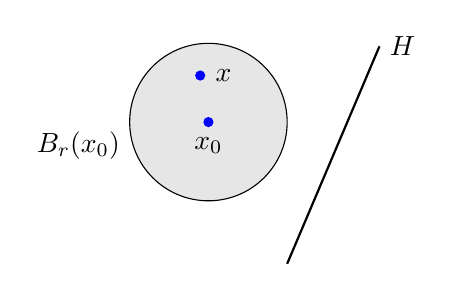
\begin{tikzpicture}[%
                mypoint/.style={shape=circle,fill=blue,inner sep=1.3pt}
        ]
            \draw [thick] (0,0) -- (67:3) node [right] {$H$};
            \fill [fill=black!50, fill opacity=0.2] (-1,1.8) circle [radius=1];
            \draw (-1,1.8) node [mypoint,label=below:$x_0$] {} circle [radius=1]
                    ++(-1,0) node [below left] {$B_r(x_0)$};
            \path (-1,1.8)++(100:0.6) node [mypoint,label=right:$x$] {};
        \end{tikzpicture}
        \caption{Hyperebene $H$ und Ball $B_r(x_0)$ um $x_0$ mit $x\in B_r(x_0)$}
        \label{vl06:fig:hyperplaneball}
    \end{figure}
    
    Wir behaupten nun, dass dann schon für alle $x\in B_r(x_0)$ die Ungleichung
    \[ \tag{$\ast$} \label{vl06:ast}
        f(x)<\alpha 
    \]
    gilt. Angenommen dies gilt nicht und es existiert ein $x_1\in
    B_r(x_0)$, so dass $f(x_1) > \alpha$ gilt. Das Segment 
    \[ [x_0,x_1] \defeq \{ x_t \defeq (1-t)\,x_0 + tx_1 \Mid t\in\I \} \]
    ist in $B_r(x_0)$ enthalten (da Bälle in normierten Räumen konvex sind).
    Somit folgt für alle $t\in\I$:
    \[ f(x_t) \neq \alpha  . \]
    Andererseits gilt offenbar
    \[ f(x_t)=\alpha \qtextq{für} t=\frac{\alpha-f(x_0)}{f(x_1)-f(x_0)} . \]
    Dies ist ein Widerspruch, also muss doch schon \eqref{vl06:ast} gelten.
    Wir erhalten, dass für alle $z\in B_1(0)$
    \[ f(\underbrace{x_0+rz}_{\in B_r(x_0)}) < \alpha  \]
    gilt, woraus sofort
    \[ f(z) < \frac{1}{r} \, \bigl( \alpha - f(x_0) \bigr) \]
    folgt. Nutze diese Ungleichung für  $z$ und $-z$ aus $B_1(0)$, um Folgendes
    für alle $z\in B_1(0)$ zu erhalten:
    \[ \abs{f(z)} < \frac{1}{r} \, \bigl( \alpha - f(x_0) \bigr)  . \]
    Insgesamt folgt:
    \[ \norm{f} = \sup_{z\in B_1(0)}\, \abs{f(z)} \leq \frac{1}{r} 
        \bigl( \alpha - f(x_0) \bigr)
    . \]
\end{proof}

% 4.10
\begin{thDef}
    Sei $X$ ein $\R$-Vektorraum und seien $A,B\subset X$ zwei Teilmengen von
    $X$. Die Hyperebene $H = \{ f=\alpha \}$ \emph{trennt die Mengen $A$ und
    $B$}, falls für alle $a\in A$ und alle $b\in B$ die Ungleichungen
    \[ f(a) \leq \alpha \qqundqq f(b) \geq \alpha \]
    gelten.
    
    \pagebreak[1]
    Die Hyperebene $H$ \emph{trennt $A$ und $B$ strikt}, falls es ein
    $\epsilon\in\R[>0]$ gibt, so dass für alle $a\in A$ und alle $b\in B$ die
    Ungleichungen
    \[ f(a) \leq \alpha-\epsilon \qqundqq f(b) \geq \alpha+\epsilon \]
    gelten.
    %
    \begin{figure}
        \centering
        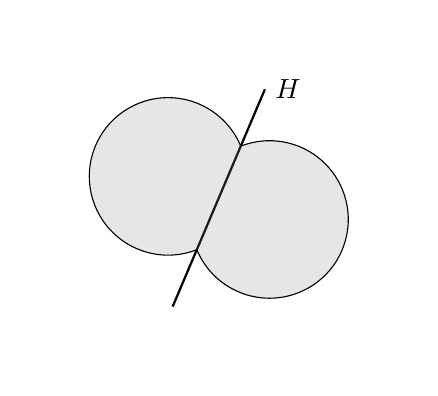
\begin{tikzpicture}[%
                rotate=-23,
                mypoint/.style={shape=circle,fill=blue,inner sep=1.3pt},
                myfill/.style={fill=black!50, fill opacity=0.2}
        ]
            \draw [thick] (0,0) -- (0,3) node [right] {$H$};
            \foreach \o in {1,-1} {
                \begin{scope}[xscale=\o]
                    \clip (0,3) rectangle (2,0);
                    \filldraw [myfill] (0.7,1.5) circle [radius=1];
                \end{scope}
            }
        \end{tikzpicture}
        \caption{Zwei \emph{nicht} strikt durch $H$ getrennte Mengen;
                 die Mengen aus \cref{vl05:fig:hyper} sind hingegen strikt
                 durch $H$ getrennt}
        \label{vl06:fig:nonstrict}
    \end{figure}
\end{thDef}

\pagebreak[2]
% 4.11
\begin{thBemerkung}\hfill
    \begin{enumerate}[i)]
        \item
            Geometrisch sagt solch eine Trennung aus, dass $A$ auf der einen
            Seite von $H$ liegt und $B$ auf der anderen Seite. (Siehe
            \cref{vl05:fig:hyper} und \cref{vl06:fig:nonstrict}.)
        \item
            Ist $X$ ein $\C$-Vektorraum, so sagen wir, dass $A$ und $B$ durch
            eine \emph{reelle Hyperebene} getrennt werden, $f\colon X\to\C$ und
            $\alpha\in\R$ existieren, so dass für alle $a\in A$ und alle 
            $b\in B$ die Ungleichungen
            \[ \Re f(x) \leq \alpha \qqundqq \Re f(b) \geq \alpha \]
            gelten. % FIXME: "analog für strikte getrennt" ?
        \item
            Wir nennen $A\subset X$ konvex, falls für alle $x,y\in A$ auch
            \[ [x,y] = \{ (1-t)\,x + ty \Mid t\in\I \} \subset A \]
            gilt.
    \end{enumerate}
\end{thBemerkung}

\nnDef\label{vl06:minkowski} Sei $X$ ein $\K$-Vektorraum und $K\subset X$. Dann ist das
\emph{Minkowski-Funktional zu $K$} definiert durch
\[ p(x) \defeq \inf\left\{ \alpha\in\R[>0] \Mid \frac{1}{\alpha}\,x \in K \right\}
. \]
% TODO: Skizze !?
Für $K=B_1(0)$ gilt gerade $p(x) = \norm{x}$.

\pagebreak[2]
% 4.12
\begin{thLemma} \label{vl06:lemma4.12}
    Es sei $K$ konvex, offen und $0\in K$. Dann gilt:
    \begin{enumerate}[i)]
        \item \label{vl06:lemma4.12:i}
            Das Minkowski-Funktional $p$ zu $K$ ist sublinear.
            
        \item \label{vl06:lemma4.12:ii}
            Es existiert ein $M\in\R[>0]$, so dass für alle $x\in X$ gilt:
            \[ 0 \leq p(x) \leq M\,\norm{x}  . \]
            
        \item \label{vl06:lemma4.12:iii}
            Zwischen $K$ und $p$ besteht folgender Zusammenhang:
            \[ K = \{ x\in X \Mid p(x) < 1 \}  . \]
    \end{enumerate}
\end{thLemma}

\begin{proof}\hfill
    \begin{enumerate}[i)]
        \item
            Seien $\lambda\in\R[>0]$ und $x\in X$. Dann gilt
            $p(\lambda x) = \lambda\, p(x)$, denn:
            \begin{align*}
                p(\lambda x) 
                &= \inf\left\{ \alpha \in\R[>0] \Mid \frac{1}{\alpha}\,\lambda x\in K \right\}
                 = \inf\left\{ \alpha'\lambda \Mid \frac{1}{\alpha'\lambda}\,
                \lambda x \in K \right\}
                \\
                &= \lambda \, \inf\left\{  \alpha' \in\R[>0] \Mid \frac{1}{\alpha'} \,
                    x \in K \right\} 
                 = \lambda\, p(x)
            \end{align*}
            Die $\triangle$-Ungleichung zeigen wir später.
            
        \item
            Es sei $r\in\R[>0]$ derart, dass $B_r(0)\subset K$ gilt. Es gilt
            dann für alle $x\in X$:
            \[ p(x) \leq \frac{1}{r} \, \norm{x} , \]
            denn:
            \begin{align*}
                p(x)
                &= \inf\left\{ \alpha\in\R[>0] \Mid \frac{1}{\alpha}\, x\in K \right\}
                \\
                &\leq \inf\left\{ \alpha\in\R[>0] \Mid \frac{1}{\alpha}\, x\in
                B_r(0) \right\}
                \\
                &= \frac{1}{r}\, \norm{x}
            \end{align*}
            
        \item
            Es sei $x\in K$. Da $K$ offen ist, folgt $(1+\epsilon)\,x\in K$ für
            $\epsilon\in\R[>0]$ klein genug. Dann gilt:
            \[ p(x) \leq \frac{1}{1+\epsilon} < 1  . \]
            Falls $p(x) < 1$ gilt, muss ein $\alpha\in(0,1)$ geben, so dass
            $x/\alpha \in K$ erfüllt ist. Damit gilt:
            \[ x = \alpha \left( \frac{x}{\alpha} \right) + (1-\alpha) \cdot 0
                \in K
            , \]
            denn $K$ ist nach Voraussetzung konvex.
            
        \item[i)]
            Es bleibt die $\triangle$-Ungleichung zu zeigen. Seien $x,y\in X$
            und $\epsilon\in\R[>0]$. Aus dem bisher Gezeigten folgt:
            \[ \frac{x}{p(x)+\epsilon}\,,\; \frac{y}{p(y)+\epsilon} \in K  . \]
            Damit gilt also für alle $t\in\I$:
            \[ \frac{tx}{p(x)+\epsilon} + \frac{(1-t)\,y}{p(y)+\epsilon} \in K
            . \]
            Wähle nun $t = \frac{p(x)+\epsilon}{p(x)+p(y)+2\epsilon}$, dann
            erhalten wir
            \[ \frac{x+y}{p(x)+p(y)+2\epsilon} \in K
                \qtextq{und mit (\ref{vl06:lemma4.12:iii} folgt}
                p\left( \frac{x+y}{p(x)+p(y)+2\epsilon} \right) < 1
            . \]
            Es folgt:
            \[ p(x+y) < p(x)+p(y)+2\epsilon  . \]
            Da $\epsilon\in\R[>0]$ beliebig war, folgt die Behauptung.
    \end{enumerate}
\end{proof}

% 4.13
\begin{thLemma} \label{vl06:lemma4.13}
    Sei $X$ ein $\K$-Vektorraum und sei $K\subset X$ nicht-leer, offen und
    konvex. Sei weiter $x_0\in K\compl$. Dann existiert ein $x'\in X'$, so
    dass für alle $x\in K$ gilt:
    \[ \Re x'(x) < \Re x'(x_0)  . \]
    Insbesondere trennt im Fall $\K=\C$ die reelle Hyperebene
    $\{ \Re x' = \Re x'(x_0) \}$ somit $\{x_0\}$ und $K$.
%    
\begin{figure}
    \centering
    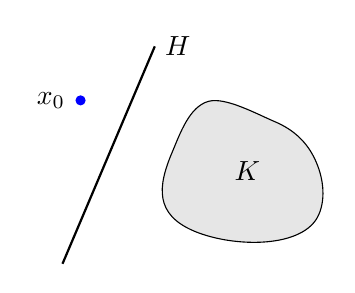
\begin{tikzpicture}[%
            rotate=-23,
            mypoint/.style={shape=circle,fill=blue,inner sep=1.3pt},
            myfill/.style={fill=black!50, fill opacity=0.2}
    ]
        \draw [thick] (0,0) -- (0,3) node [right] {$H$};
        
        \begin{scope}[shift={(-0.2,-0.2)}]
        \begin{scope}[y=0.4pt, x=0.4pt]
            \filldraw [myfill] 
                (210.0000,145.8622) .. controls (210.0000,162.7022) and
                (199.8512,178.9613) .. (187.4601,190.0677) .. controls (174.8589,201.3623) and
                (159.8532,207.3622) .. (140.5000,207.3622) .. controls (122.6292,207.3622) and
                (90.5838,210.6436) .. (78.2706,200.8363) .. controls (64.1369,189.5790) and
                (66.0503,163.8372) .. (66.0503,145.6854) .. controls (66.0503,111.7199) and
                (73.6162,87.8622) .. (112.0000,87.8622) .. controls (150.3838,87.8622) and
                (210.0000,111.8967) .. (210.0000,145.8622) -- cycle;
        \end{scope}
        \end{scope}
        
        \path (-0.6,2) node [mypoint,label=left:$x_0$] {};
        \path (1.7,2) node {$K$};
    \end{tikzpicture}
    %
    \hspace{3cm}
    %
    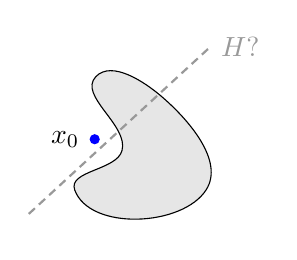
\begin{tikzpicture}[%
            rotate=-23,
            mypoint/.style={shape=circle,fill=blue,inner sep=1.3pt},
            myfill/.style={fill=black!50, fill opacity=0.2}
    ]
        \begin{scope}[shift={(0,-0.8)}]
        \begin{scope}[y=0.4pt, x=0.4pt]
            \filldraw [myfill] 
                (181.7157,97.0718) .. controls (186.6559,127.6093) and
                (141.6761,149.1361) .. (112.2157,158.5718) .. controls (92.3528,164.9336) and
                (57.3842,171.5468) .. (49.9863,152.0460) .. controls (41.6006,129.9411) and
                (94.7512,123.1588) .. (97.8701,99.7235) .. controls (100.3116,81.3774) and
                (59.8005,63.9407) .. (72.4020,50.3855) .. controls (99.3796,21.3664) and
                (175.3882,57.9584) .. (181.7157,97.0718) -- cycle;
        \end{scope}
        \end{scope}
        
        \draw [thick, color=black!40, densely dashed] 
            (0.6,-0.6) -- (50:2.95) node [right] {$H$?};
        
        \path (1,0.6) node [mypoint,label=left:$x_0$] {};
    \end{tikzpicture}
    \caption{Links eine konvexe Menge~$K$, getrennt von $\{x_0\}$ durch $H$;
             rechts eine nicht konvexe Menge, so dass diese und $x_0$ nicht
             durch eine Hyperebene~$H$ getrennt werden können}
    \label{vl06:fig:convexvsnonconvex}
\end{figure}
\end{thLemma}

\begin{proof}
    Sei zunächst $\K=\R$.  Ohne Einschränkung können wir $0\in K$ annehmen. Sei
    $p$ das Minkowski-Funktional zu $K$. Sei weiter $U\defeq\spann\{x_0\}$ und
    $g\colon U\to\R$ sei gegeben durch $g(tx_0) \defeq t$ für alle $t\in\R$.
    Dann gilt für alle $x\in U$:
    \[ g(x) \leq p(x) \]
    und für $x_0$ haben wir $g(x_0) = 1 \leq p(x_0)$, da $x_0$ nicht in $K$
    liegt. (Achtung: $tx_0$ mit $t<0$ ist kein Problem, da $g(tx_0)<0$.)
    
    Wende nun Hahn-Banach \pcref{vl05:hahnbanach} an, womit wir ein $x'\colon
    X\to\R$ erhalten, mit $x'(x)\leq p(x)$ für alle $x\in X$ und außerdem
    $x'\vert_U = g$. Insbesondere gilt also $x'(x_0)=1$. Außerdem ist
    $x'$ stetig (vgl. \mycrefA{vl06:lemma4.12:ii}{}{\,(}{}).
    Mit \mycrefA{vl06:lemma4.12:iii}{}{\,(}{} erhalten wir: für alle $x\in K$
    gilt
    \[ x'(x) < 1  . \]
    %
    Der komplexe Fall (also $\K=\C$) folgt aus dem Obigen und
    \cref{vl05:lemma4.4}.
    \\
\end{proof}

% 4.14
\begin{thSatz}[Satz von Hahn-Banach (erste geometrische Formulierung)]
    \label{vl06:hahnbanachgeom1}
    %
    Sei $X$ ein normierter $\K$-Vektorraum und seien $A,B\subset X$ nicht-leer,
    konvex und disjunkt. Außerdem sei $A$ offen.
    Dann existiert $x'\in X'$ mit $\Re x'(a) < \Re x'(b)$ für alle $a\in A$ und
    $b\in B$.
\end{thSatz}

Bemerkung: Ist $X$ ein $\R$-Vektorraum, so trennt die abgeschlossene Hyperebene
$\{ x'=\alpha \}$ mit 
\[ \alpha\in \bigl[ \sup_{a\in A} x'(a), \inf_{b\in B} x'(b) \bigr] \]
die Mengen $A$ und $B$.

\begin{proof}
    Es sei $C\defeq A-B \defeq \{ a-b \Mid a\in A,\, b\in B \}$. Dann ist $C$
    konvex (leichte Rechnung) und offen, denn:
    \[ C = \bigcup_{b\in B} \underbrace{ (A-\{b\}) }_{\text{offen}}  . \]
    Da $A$ und $B$ disjunkt sind, liegt $0$ nicht in $C$.
    Aus \cref{vl06:lemma4.13} folgt die Existenz eines $x'\in X'$, welches für
    alle $x\in C$ die Ungleichung
    \[ \Re x'(x) < 0 = \Re x'(0) \]
    erfüllt. Das heißt, es gilt für alle $a\in A$ und $b\in b$
    \begin{gather*}
        \Re x'(a-b) < 0 \qtextq{oder äquivalent}
        \Re x'(a) < \Re x'(b)
        . 
        \\
        \qedhere
    \end{gather*}
\end{proof}

% 4.15
\begin{thSatz}[Satz von Hahn-Banach (zweite geometrische Formulierung)]
    \label{vl06:hahnbanachgeom2}
    %
    Sei $X$ ein normierter $\K$-Vektorraum und seien $A,B\subset X$ nicht-leer,
    konvex und disjunkt. Weiter sei $A$ abgeschlossen und $B$ kompakt.  Dann
    exisistiert ein $x'\in X'$ sowie ein $\alpha\in\R$ und ein
    $\epsilon\in\R[>0]$, so dass für alle $a\in A$ und $b\in B$ die
    Ungleichungen
    \[ \Re x'(a) + \epsilon \leq \alpha \leq \Re x'(b) - \epsilon \] 
    gelten.
\end{thSatz}

\begin{proof}
    Es sei $C\defeq A-B$ wie bei \cref{vl06:hahnbanachgeom1}.
    Damit ist $C$ konvex und abgeschlossen (siehe unten) % TODO: future ref
    und es gilt $0\notin C$. Damit existiert ein $r\in\R[>0]$, so dass
    $B_r(0) \cap C = \emptyset$ gilt.
    \cref{vl06:hahnbanachgeom1} liefert: Es existiert ein $x'\in X'$ mit
    $x'\not\equiv 0$, so dass für alle $a\in A,\, b\in B$ und $z\in B_1(0)$ gilt:
    \[ \Re x'(a-b) < \Re x'(rz) . \]
    Also gilt für alle $a\in A$ und $b\in B$:
    \[ \Re x'(a-b) \leq -r\,\norm{x'}  . \]
    Für $\epsilon r\norm{x'}/2 > 0$ ergibt sich, dass für alle $a\in A$ und
    alle $b\in B$ gilt:
    \[ \Re x'(a) + \epsilon \leq \Re x'(b) - \epsilon . \]
    Wähle $\alpha\in\R[>0]$, so dass
    \[ \sup_{a\in A} \, \bigl( x'(a) + \epsilon \bigr) \leq \alpha 
        \leq \sup_{b\in B} \, \bigl( x'(b) - \epsilon \bigr)
    \]
    erfüllt ist. Noch zu zeigen: $C$ ist abgeschlossen.
    Sei $\nSeq c = (a_n-b_n)_{n\in\N}$ eine Folge in $C$ mit Grenzwert $c\in X$.
    Da $B$ kompakt ist, existiert eine Teilfolge $(b_{n_k})_{k\in\N}$ 
    von $\nSeq b$, mit $b_{n_k} \to b\in B$ für $k\to\infty$. Damit ergibt
    sich: 
    \[ a_{n_k} = c_{n_k} + b_{n_k} \ntoinfty c + b  . \]
    Da $A$ abgeschlossen ist, folgt $c+b\in A$ und damit $c = (c+b)-b \in A-B=C$.
    \\
\end{proof}
